\documentclass[../Отчет.tex]{subfiles}

\begin{document}
  \section{Архитектура системы}
  \par
  Архитектура системы требуется для упрощения поддержки и модификации продукта в долгосрочной перспективе. Правильное разделение на модули упрощает выделение сущностей, их переиспользование.
  \subsection{Backend}
  \par
  Для backend части выбран традиционный для фреймворка Laravel паттерн Model-View-Controller, с выделением дополнительных слоев бизнес-логики (Services).
  \begin{figure}[H]
    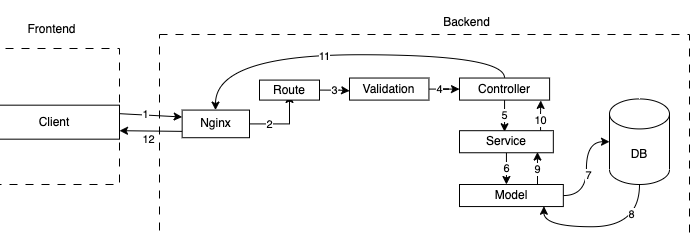
\includegraphics[width=\textwidth, frame]{../graphics/uml-back.png}
    \caption{Схема backend архитектуры}
    \label{pic:backarch}
  \end{figure}
  \begin{enumerate}
    \item Клиент отправляет запрос на сервер.
    \item Запрос обрабатывается Nginx (или другим сервером).
    \item Проверяется путь запроса с помощью класса Route, вызывается метод связанного с путем Controller.
    \item Происходит валидация запроса, объект с информацией о запросе попадает в Controller.
    \item Controller вызывает методы связанных с ним Service - классов.
    \item Service класс вызывает методы связанных с ним классов Model.
    \item Model получает данные из базы данных.
    \item Model возвращает данные в Service.
    \item Service возвращает результирующий объект с данными.
    \item Controller возвращает ответ с полученными данными.
  \end{enumerate}
  \begin{itemize}
    \item Route — класс, связывающий URL, допустимые HTTP-методы для него и метод контроллера, вызываемый при запросе по указанному URL.
    \item Controller — класс, содержащий методы для обработки запросов. Для каждого Controller существует Service и Model.
    \item Service — класс, содержащий в себе методы для работы с соответствующими Model. Чаще всего это операции чтения, удаления, вставки.
    \item Model — класс, связаннный с конкретной таблице в базе данных. Позволяет запрашивать данные из этой таблицы. Наследуется от базового класса Model из Eloquent ORM.
  \end{itemize}
  \subsection{Frontend}
  \par 
  Для frontend части достаточно разделения на компоненты (компоненты интерфейса и компоненты взаимодействующие с бизнес-логикой). Из компонентов собираются страницы, с использованием layout компонентов.
  Так как за хранение состояния приложения и работу с данными отвечает сервер, проектирование хранилища глобального состояния приложения не требуется.
  \clearpage
\end{document}